\documentclass[10pt,twocolumn]{article}
\usepackage[margin=0.56in,top=0.60in,bottom=0.60in]{geometry}
\usepackage{amsmath,amssymb,amsthm}
\usepackage{booktabs}
\usepackage{graphicx}
\usepackage{microtype}
\usepackage[hidelinks]{hyperref}
\usepackage{xurl}

\raggedbottom
\setlength{\columnsep}{0.20in}
\setlength{\parskip}{1.5pt}
\setlength{\textfloatsep}{7pt plus 2pt minus 2pt}
\setlength{\dbltextfloatsep}{8pt plus 2pt minus 2pt}

\title{\vspace{-1.2em}\textbf{Exact Rational and Constructive Lean~4 Certificates for Non-Additivity of Extension Complexity Under Cartesian Products}\vspace{-0.4em}}
\author{Lluis Eriksson\\
\small Independent Researcher (\nolinkurl{https://github.com/lluiseriksson})\\
\small Companion Preprint to Minhao Liu (\texttt{arXiv:2611.33631v1}) --- Unrefereed Formal-Verification Artifact\vspace{-0.6em}}
\date{November 26, 2026}

\begin{document}
\maketitle

\begin{abstract}
\noindent Minhao Liu (\texttt{arXiv:2611.33631v1}, Nov.~2026) disproves Conjecture~1.2 of Grande, Padrol, and Sanyal by proving that linear extension complexity is not additive under Cartesian products: an explicit 24-dimensional rational polytope $P$ with 50 facets and 150 vertices satisfies $\mathrm{xc}(P)=40$ and $\mathrm{xc}(P\times P)=79$, while infinite families $(U_n, V_n)$ and Cartesian squares $R_t \times R_t$ achieve linear-fraction deficits $\delta(U_n,V_n)\ge\lceil 5n/27\rceil$ and unbounded square deficits $\delta(R_t,R_t)\ge t$. Because neither ordinary rank nor rectangle covering detects the subadditivity gap---requiring exact facet-wedge lifting, magnitude-sensitive probe/alternating-sum inequalities, conditional label-profile counting, and alphabet-separated cover numbers---we present an independent companion verification artifact (\texttt{EXT-COMPLEXITY-PROD-CERT-1.0}) containing: (i)~18 constructive theorems in Lean~4.35.0 (zero \texttt{sorry}, zero custom axioms, zero \texttt{Classical.choice}); (ii)~a zero-floating-point Python verifier over exact $\mathbb{Z}$ and $\mathbb{Q}$ checking four verification modes (eight submodes); and (iii)~16 canonical JSON certificates (\texttt{C01}--\texttt{C16}) and 43 unit/forgery tests auditing every exact matrix factorization, facet/vertex count, and quantitative threshold.
\end{abstract}

\section{Introduction and Scope}
By Yannakakis' factorization theorem~\cite{Yannakakis1991}, the linear extension complexity $\mathrm{xc}(Q)$ of a polytope $Q$ equals the nonnegative rank $\mathrm{rank}_+ S_Q$ of its slack matrix, and the slack matrix of a Cartesian product $Q\times Q'$ is the 1-product $S_Q \otimes_1 S_{Q'}$~\cite{AprileEtAl2024,ConfortiCornuejolsZambelli2013}. While $\mathrm{xc}(Q\times Q') \le \mathrm{xc}(Q)+\mathrm{xc}(Q')$ is immediate and equality holds when one factor is a simplex~\cite{GrandePadrolSanyal2018} or a pyramid~\cite{TiwaryWeltgeZenklusen2017}, whether additivity holds in general (Conjecture~1.2 of~\cite{GrandePadrolSanyal2018}) remained open since the 2013 Dagstuhl seminar. In~\cite{Liu2026ExtensionComplexity}, Minhao Liu resolves the question negatively, echoing strict subadditivity of tensor rank~\cite{Shitov2019} and positive semidefinite rank~\cite{GouveiaRobinsonThomas2013}.

\paragraph{Scope and attribution.}
This paper is an \emph{unrefereed companion verification preprint} to~\cite{Liu2026ExtensionComplexity}. All mathematical theorems, polytope constructions, and proof techniques belong exclusively to Minhao Liu~\cite{Liu2026ExtensionComplexity}. Our contribution is an independent, deterministic, zero-floating-point audit layer checking the finite algebraic, polyhedral, and quantitative pillars of~\cite{Liu2026ExtensionComplexity} in Lean~4.35.0 and exact rational Python. General real-valued conic factorizations are treated in~\cite{Liu2026ExtensionComplexity} via the quantitative probe and counting inequalities that we mechanize and verify here.

\section{Constructive Lean~4 Formalization}
We formalize 18 core theorems of~\cite{Liu2026ExtensionComplexity} in \nolinkurl{lean/ExtensionComplexityCert.lean} under Lean~4.35.0 without Mathlib. Every theorem is audited via \texttt{\#print axioms} to depend exclusively on \texttt{propext} and \texttt{Quot.sound} (zero \texttt{sorry}, zero custom axioms, zero \texttt{Classical.choice}, zero compiler warnings). Table~\ref{tab:lean} summarizes the 18 theorems.

\begin{table}[t]
\centering
\scriptsize
\setlength{\tabcolsep}{2.2pt}
\caption{Constructive Lean~4.35.0 theorems in \texttt{ExtensionComplexityCert.lean} (18/18 built, 0~\texttt{sorry}, 0~\texttt{Classical.choice}).}
\label{tab:lean}
\begin{tabular}{@{}cll@{}}
\toprule
\# & Lean Theorem Group & Paper Pillar~\cite{Liu2026ExtensionComplexity} \\
\midrule
1--2 & \texttt{thm3\_wedge\_*}, \texttt{lemma5\_wedge\_*} & Sec.~2 Thm.~3 \& Lem.~5 \\
3 & \texttt{thm1\_polytope\_P\_exact\_counts} & Thm.~1 ($\dim 24,50,150,40,79$) \\
4--7 & \texttt{prop9\_claim2\_*}, \texttt{claim3\_*}, \texttt{claim4\_*} & Sec.~4 Prop.~9 Claims~1--4 \\
8 & \texttt{prop10\_base\_B\_facet\_and\_vertex\_*} & Sec.~5 Prop.~10 ($37,39,13$) \\
9--11 & \texttt{prop11\_incidence\_*}, \texttt{discrete\_*} & Sec.~6.2 Prop.~11 ($c_2,c_3$) \\
12--13 & \texttt{thm2\_linear\_*}, \texttt{sec62\_frac\_*} & Sec.~6.2--6.3 ($\delta\ge\tfrac{5n}{27}$) \\
14--16 & \texttt{lemma12\_*}, \texttt{lemma13\_*}, \texttt{square\_*} & Sec.~6.4 Lem.~12--13 ($\delta\ge t$) \\
17--18 & \texttt{sec7\_corollaries\_*}, \texttt{sec72\_*} & Sec.~7 Cor.~14--15 \& $8\to 7$b \\
\bottomrule
\end{tabular}
\end{table}

Three constructive highlights anchor the mechanization. First, Theorems~4--6 certify Liu's exact rational Proposition~9 bounds with zero floating-point rounding: $26(\tau+2\beta) = \tfrac{663}{2500} < 1$ (Claim~2) and $26\max(6\beta, \tfrac{6\varepsilon}{1-\varepsilon}) = \tfrac{62412}{76523} < 1$ (Claim~3, via $13\cdot 62412 = 811356 < 994799 = 13\cdot 76523$), while Theorem~5 proves universally over $\mathbb{N}$ that deficient-node budgets exceed $13d$ for $d\in\{1,2\}$. Second, Theorems~9--12 mechanize Proposition~11's incidence-and-good-block combination at $N=6$, proving $27(r_2+r_3-r_{\mathrm{joint}}) \ge 5n$ from $r_2 \ge (p+3)n$, $27r_3 \ge (27p+32)n$, and $r_{\mathrm{joint}} \le (2p+4)n$, together with the discrete ratio test establishing $\max_{d\ge 1} d(3/4)^{d-1} = 27/16$ at $d\in\{3,4\}$. Third, Theorems~14--16 formalize all three cases of Lemma~12's cover additivity $C_t = C + j$ ($j \ge 2C$), Lemma~13's $N^\star = D+q$ budget cancellation, and an inductive proof over arbitrary lists $[j_1,\dots,j_t]$ ($j_i \ge 1$) that $2\sum j_i - \sum(2j_i-1) = t$.

\section{Zero-Float Verifier Architecture}
Our verifier \nolinkurl{src/ext_complexity_verifier.py} is audited by AST inspection for zero \texttt{float} literals, zero \texttt{float()} calls, zero true-division operators (\texttt{/}, \texttt{/=}), and zero \texttt{math}/\texttt{numpy} imports. Rationals are encoded as lowest-terms pairs $[a,b]$ with pre-read \texttt{is\_file()}/\texttt{st\_size} $\le 10^6$-byte guards, duplicate-key rejection, non-finite constant rejection, and recursion trapping. Four verification modes cover all sections of~\cite{Liu2026ExtensionComplexity}:

\begin{enumerate}\itemsep 1.5pt
\item \textbf{Mode~1 (\nolinkurl{wedge_transfer_and_slack_polytope}):} Submode~1a checks Lemma~5's zero-pattern condition ($\forall$ nonzero row $g$, $\exists i: M_{gi}=0<\sigma_i$) and verifies that a nonnegative factorization $M=UV$ of rank $r$ lifts identically to $M_\sigma = U_\sigma V_\sigma$ of rank $r+2$. Submode~1b builds the twin-hexagon graph $G$, checks $\mathrm{rank}_{\mathbb{Q}}(R)=11$ and $R\kappa=0$, verifies $X_t = X_0 + R b_t$, validates all 37 facets of $B$ via explicit single-tight-facet witnesses, checks rank-11 tight subsystems for all 39 vertices of $B$, and verifies the 13-wedge lift $P=\hat{B}$ has $\dim P=24$, 50 facets, and $3\cdot 2+36\cdot 4=150$ vertices.
\item \textbf{Mode~2 (\nolinkurl{six_cycle_subadditivity_and_bounds}):} Submode~2a constructs the $24\times 39$ matrix $S$, verifies $\mathrm{rank}_{\mathbb{Q}}(S)=12$ (Remark~8), certifies Lemma~7's 14-generator nonnegative factorization of $S$ and 27-generator nonnegative factorization of $S\otimes_1 S$ across all $39^2 = 1{,}521$ pairs ($73{,}008$ exact integer entries), and verifies Eq.~(4.1) ($D(R_v)=0$, $D(A_s)=D(X_t)=1$) across all $2^6 = 64$ six-cycles of $G$. Submode~2b checks Proposition~9's exact rational Claim~2 and Claim~3 bounds.
\item \textbf{Mode~3 (\nolinkurl{linear_fraction_deficit_Un_Vn}):} Submode~3a constructs $\Gamma_2$ and $\Gamma_3$, verifies $T\cap U\neq\emptyset$ across all $24$ pairs in $\mathcal{T}_2\times\mathcal{T}_3$, checks Eq.~(6.1) for all $(T,s)$, and computes exact $\mathbb{Q}$-ranks before and after deleting $I(f)$ for every coarse node $f$ (Sec.~6.3), proving every coordinate inequality is a distinct facet. Submode~3b checks Proposition~11's scale parameters, discrete maxima ($1$ and $27/16$), 3-block fractional relaxation ($64/18=32/9$), and exact deficit $\delta(U_n,V_n)\ge\lceil 5n/27\rceil$.
\item \textbf{Mode~4 (\nolinkurl{unbounded_square_and_corollaries}):} Submode~4a verifies Lemma~12's growth condition $j_i \ge 2\sum_{h<i}j_h$, pairwise intersection of $\mathcal{F}_{j_i}$, Lemma~13's exact parameters $(D,q,s^\star,N^\star,p^\star,H)$ and perfect-square scale $\Lambda = (\sqrt{\Lambda})^2$, and square deficit $t$. Submode~4b checks Corollaries~14--15, the Sec.~7.1 face bound $0\le\delta\le 16$, and Sec.~7.2's zero-error channel bit-width drop~\cite{CohenRothblum1993}.
\end{enumerate}

\section{Canonical Certificates and Worked Witnesses}
All 16 canonical certificates (\texttt{C01}--\texttt{C16}) verify deterministically via \nolinkurl{python -m src.ext_complexity_verifier certificates}, and all 43 tests in \nolinkurl{tests/test_verifier.py} pass in $0.95\,\mathrm{s}$. Table~\ref{tab:certs} summarizes the live outputs.

\begin{table*}[t]
\centering
\scriptsize
\setlength{\tabcolsep}{4.0pt}
\caption{Summary of all 16 verified \texttt{EXT-COMPLEXITY-PROD-CERT-1.0} canonical certificates (\texttt{C01}--\texttt{C16}), with exact outputs from \texttt{verify\_file}.}
\label{tab:certs}
\begin{tabular}{@{}llll@{}}
\toprule
ID & Mode / Submode & Input Instance & Exact Certified Metrics \\
\midrule
\texttt{C01} & M1a Wedge Lift & Pentagon $M_{4\times 5}$, omitted $\sigma$ & Lemma~5 holds on 4/4 rows; lifted $M_\sigma$ is $6\times 10$, rank $4\to 6$ \\
\texttt{C02} & M1a Wedge Lift & Prism $M_{4\times 6}$, scaled $U,V$ & Lemma~5 holds on 4/4 rows; lifted $M_\sigma$ is $6\times 12$, rank $4\to 6$ \\
\texttt{C03} & M1b Polytope $P$ & Canonical $L=10^6$ & $\mathrm{rank}(R)=11$, $B$: $37$ facets/$39$ verts; $P$: $\dim 24, 50, 150$ \\
\texttt{C04} & M1b Polytope $P$ & Scaled $L=10^7$ & Exact scale invariance: $B$ ($37,39$) $\to$ $P$ ($\dim 24, 50, 150$) \\
\texttt{C05} & M2a Twin-Hex $S$ & Canonical $L=10^6$ & $\mathrm{rank}(S)=12$, $\mathrm{rank}_+\le 14$, $\mathrm{rank}_+(S\otimes_1 S)\le 27$, $1521$ pairs, $64$ cycles \\
\texttt{C06} & M2a Twin-Hex $S$ & Scaled $L=5\cdot 10^6$ & Exact $14$/$27$ nonnegative factorizations across $73{,}008$ entries \\
\texttt{C07} & M2b Prop.~9 & $L=10^6$, $\tau=\tfrac{1}{5000}$ & Claim~2 UB $\tfrac{663}{2500}\approx 0.2652<1$; Claim~3 UB $\tfrac{62412}{76523}\approx 0.8156<1$ \\
\texttt{C08} & M2b Prop.~9 & $L=10^7$, $\tau=\tfrac{1}{20000}$ & Claim~2 UB $\tfrac{1053}{10000}=0.1053<1$; Claim~3 UB $\approx 0.3120<1$ \\
\texttt{C09} & M3a Dict./Facets & $\Gamma_2, \Gamma_3$, $N=6$ & $p=72$, rows $1080/1728$, $\mathrm{rank}(E_2)=9$, $\mathrm{rank}(E_3)=7$, all drops $=1$ \\
\texttt{C10} & M3a Dict./Facets & $\Gamma_2, \Gamma_3$, $N=8$ & $p=96$, rows $2432/4096$, exact Sec.~6.3 node-deletion rank drop \\
\texttt{C11} & M3b Prop.~11 & $n=6, N=6$ (Sec.~6.2) & $\mathrm{rank}_+ M_{2,6}=450$, $\mathrm{rank}_+ M_{3,6}\ge 440$, joint $\le 888$, $\delta\ge 2$ \\
\texttt{C12} & M3b Prop.~11 & $n=27, N=6$ & $\mathrm{rank}_+ M_{2,27}=2025$, $\mathrm{rank}_+ M_{3,27}\ge 1976$, joint $\le 3996$, $\delta\ge 5$ \\
\texttt{C13} & M4a Squares & $t=2$, $j=[2,4]$, $\sqrt{\Lambda}=10^{10}$ & $C_2=6$, $N^\star=24$, $p^\star=3504$, $1234$ pair checks, $\delta(R_2,R_2)\ge 2$ \\
\texttt{C14} & M4a Squares & $t=2$, $j=[2,5]$, $\sqrt{\Lambda}=10^{14}$ & $C_2=7$, $N^\star=75$, $p^\star=47700$, $\delta\ge 2$, Lemma~13 bounds $<1$ \\
\texttt{C15} & M4b Cor./Channel & $d_{\mathrm{chan}}=48$ ($\Delta_{48}$) & Cor.~14--15 exact; $129\to 128$ messages ($8\to 7$ bits saved!) \\
\texttt{C16} & M4b Cor./Channel & $d_{\mathrm{chan}}=176$ ($\Delta_{176}$) & Cor.~14--15 exact; $257\to 256$ messages ($9\to 8$ bits saved!) \\
\bottomrule
\end{tabular}
\end{table*}

\begin{figure*}[t]
\centering
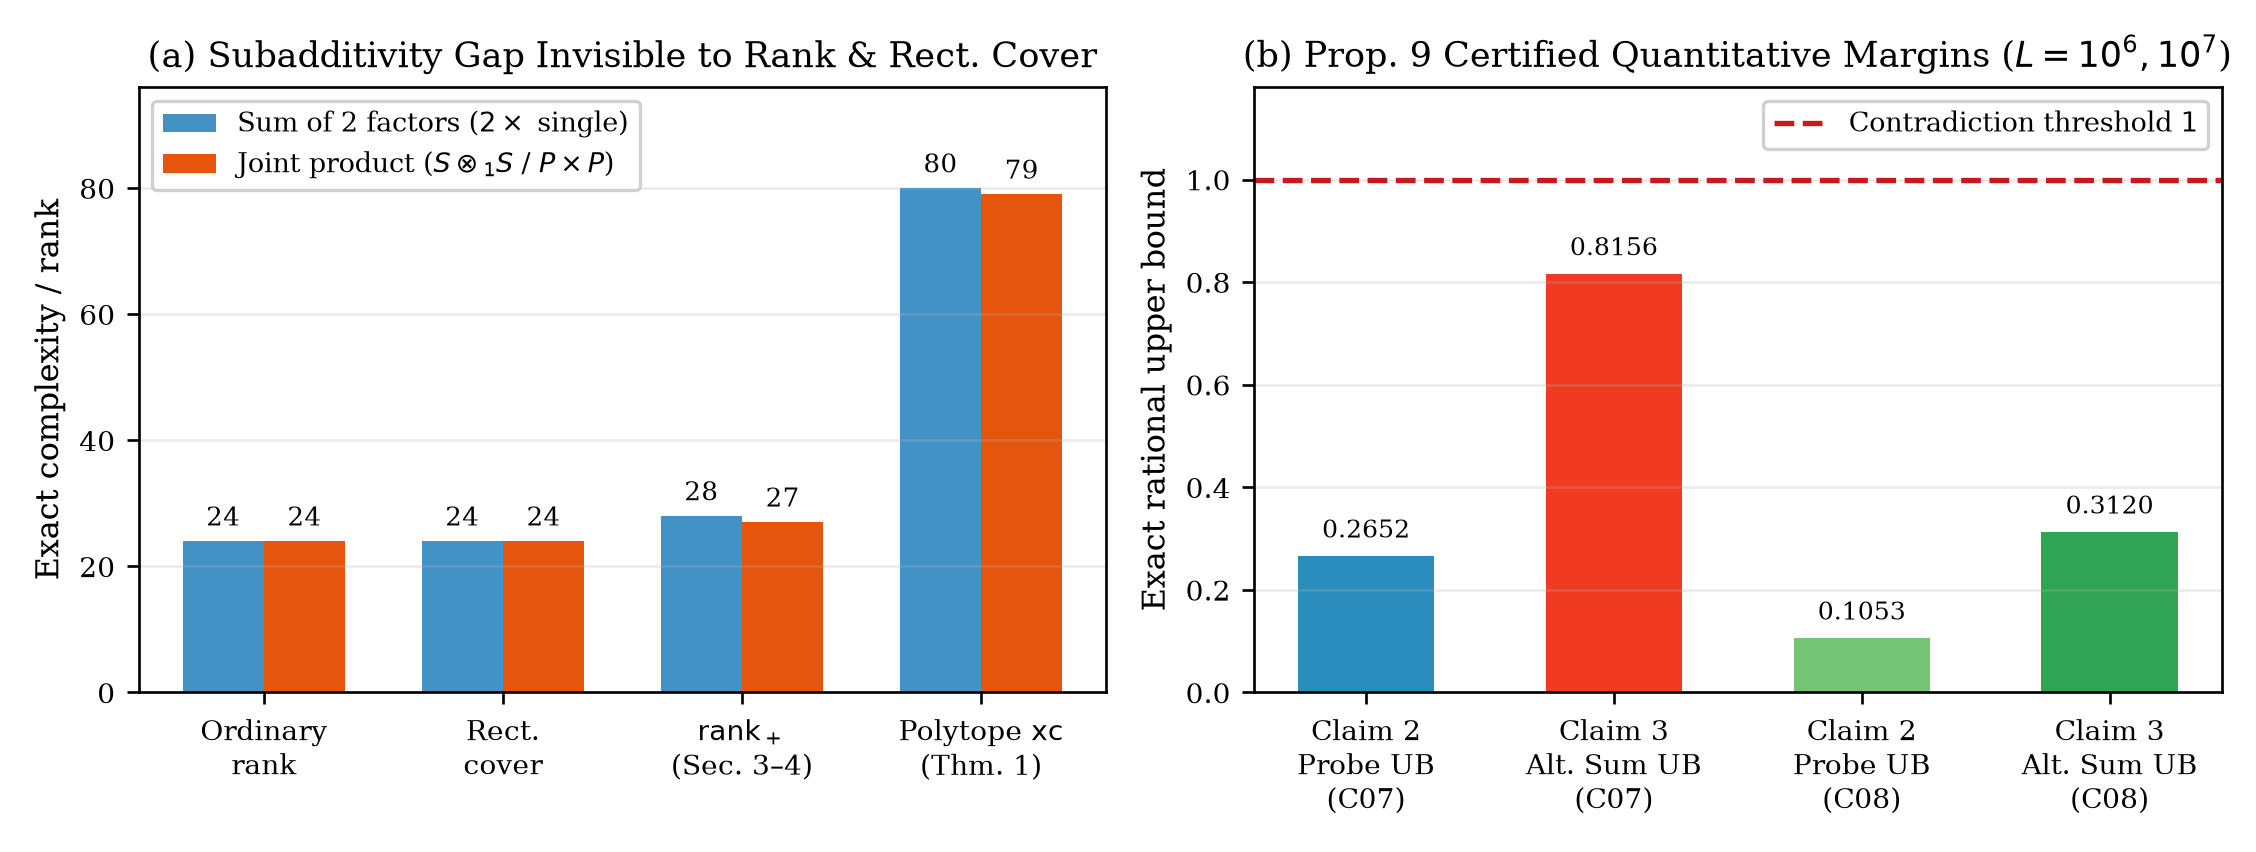
\includegraphics[width=0.90\textwidth]{figures/fig1_rank_gap_and_prop9_margins.png}
\caption{\textbf{Theorem~1 Subadditivity Gap and Proposition~9 Margins.} (a)~Ordinary rank and rectangle cover cap at $24$ for both $2\times$ single and joint products, whereas exact $\mathrm{rank}_+$ drops from $28$ to $27$ and polytope $\mathrm{xc}$ drops from $80$ to $79$ (\texttt{C03}, \texttt{C05}). (b)~Certified rational Proposition~9 upper bounds strictly below $1$ (\texttt{C07}, \texttt{C08}).}
\label{fig:fig1}
\end{figure*}

\begin{figure*}[t]
\centering
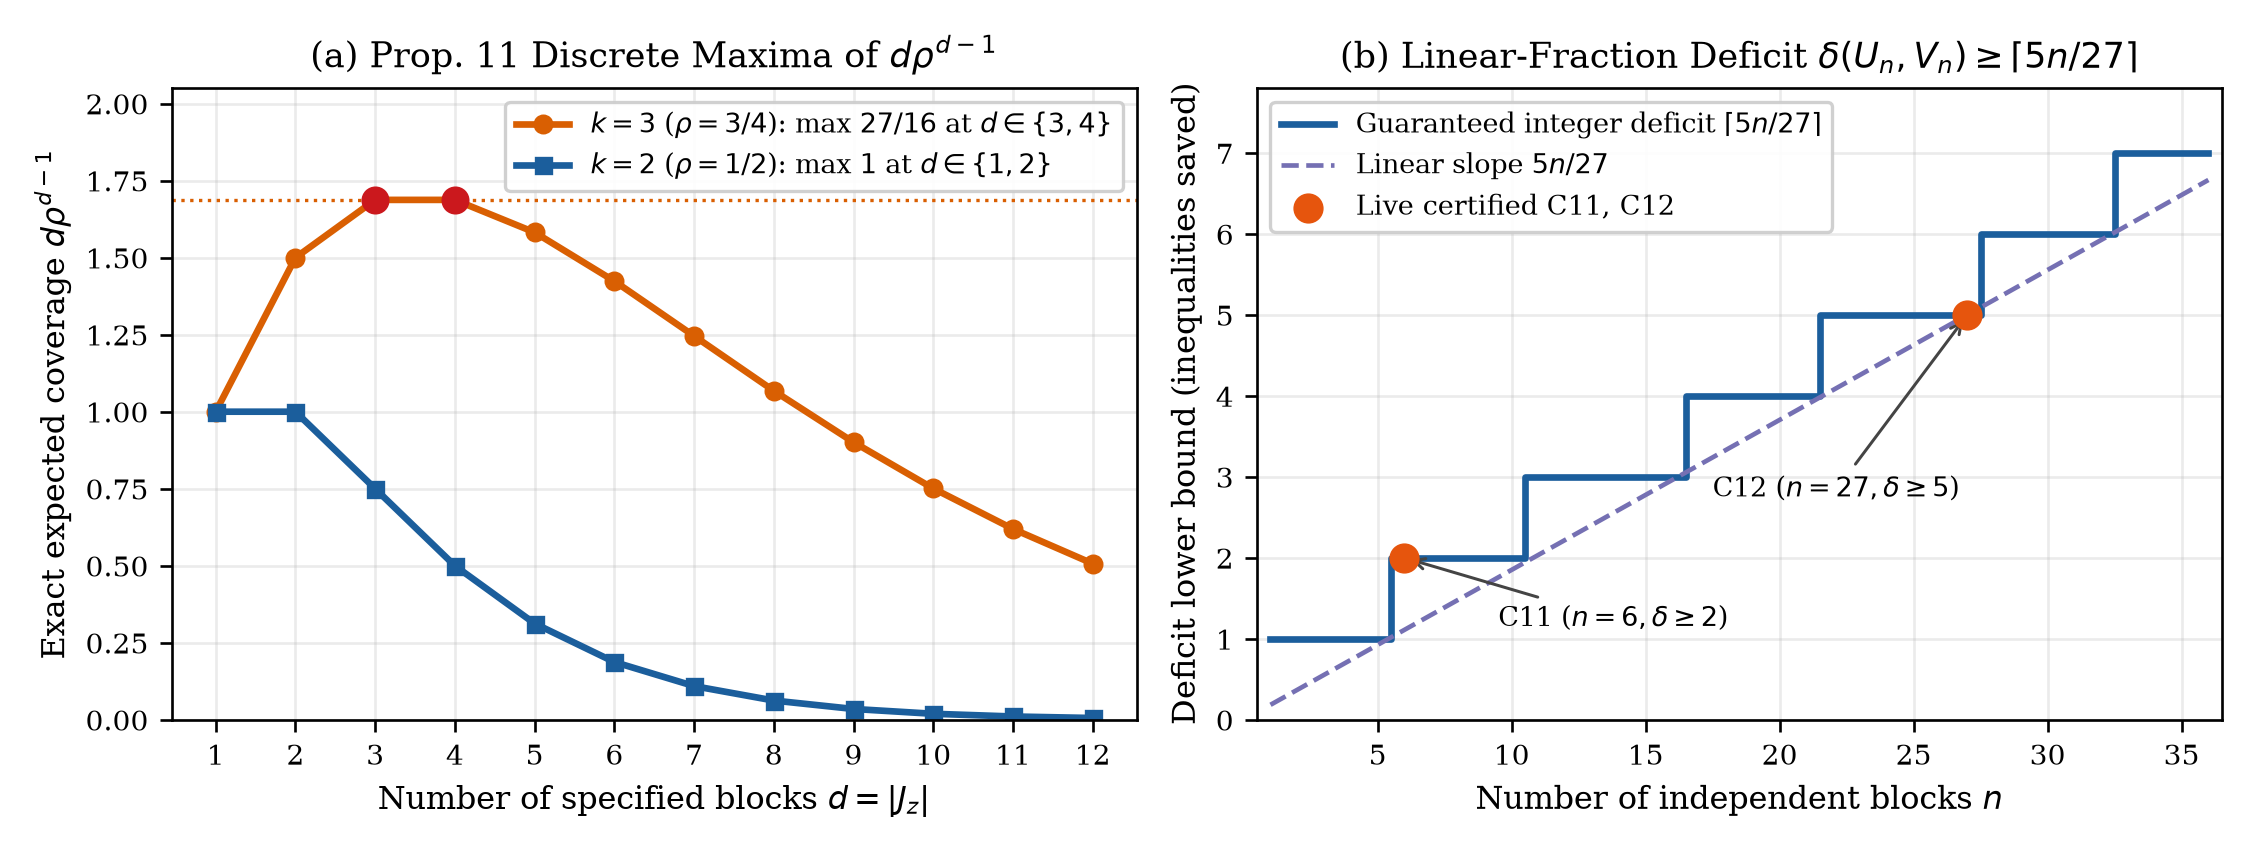
\includegraphics[width=0.90\textwidth]{figures/fig2_prop11_counting_and_deficit.png}
\caption{\textbf{Linear-Fraction Deficit Construction (Sec.~6.1--6.3).} (a)~Exact discrete maxima of $d\rho^{d-1}$ at $\rho=1/2$ (max $1$) and $\rho=3/4$ (max $27/16$ at $d\in\{3,4\}$). (b)~Guaranteed integer deficit $\delta(U_n,V_n)\ge\lceil 5n/27\rceil$ with live certified instances \texttt{C11} ($n=6, \delta\ge 2$) and \texttt{C12} ($n=27, \delta\ge 5$).}
\label{fig:fig2}
\end{figure*}

\begin{figure*}[t]
\centering
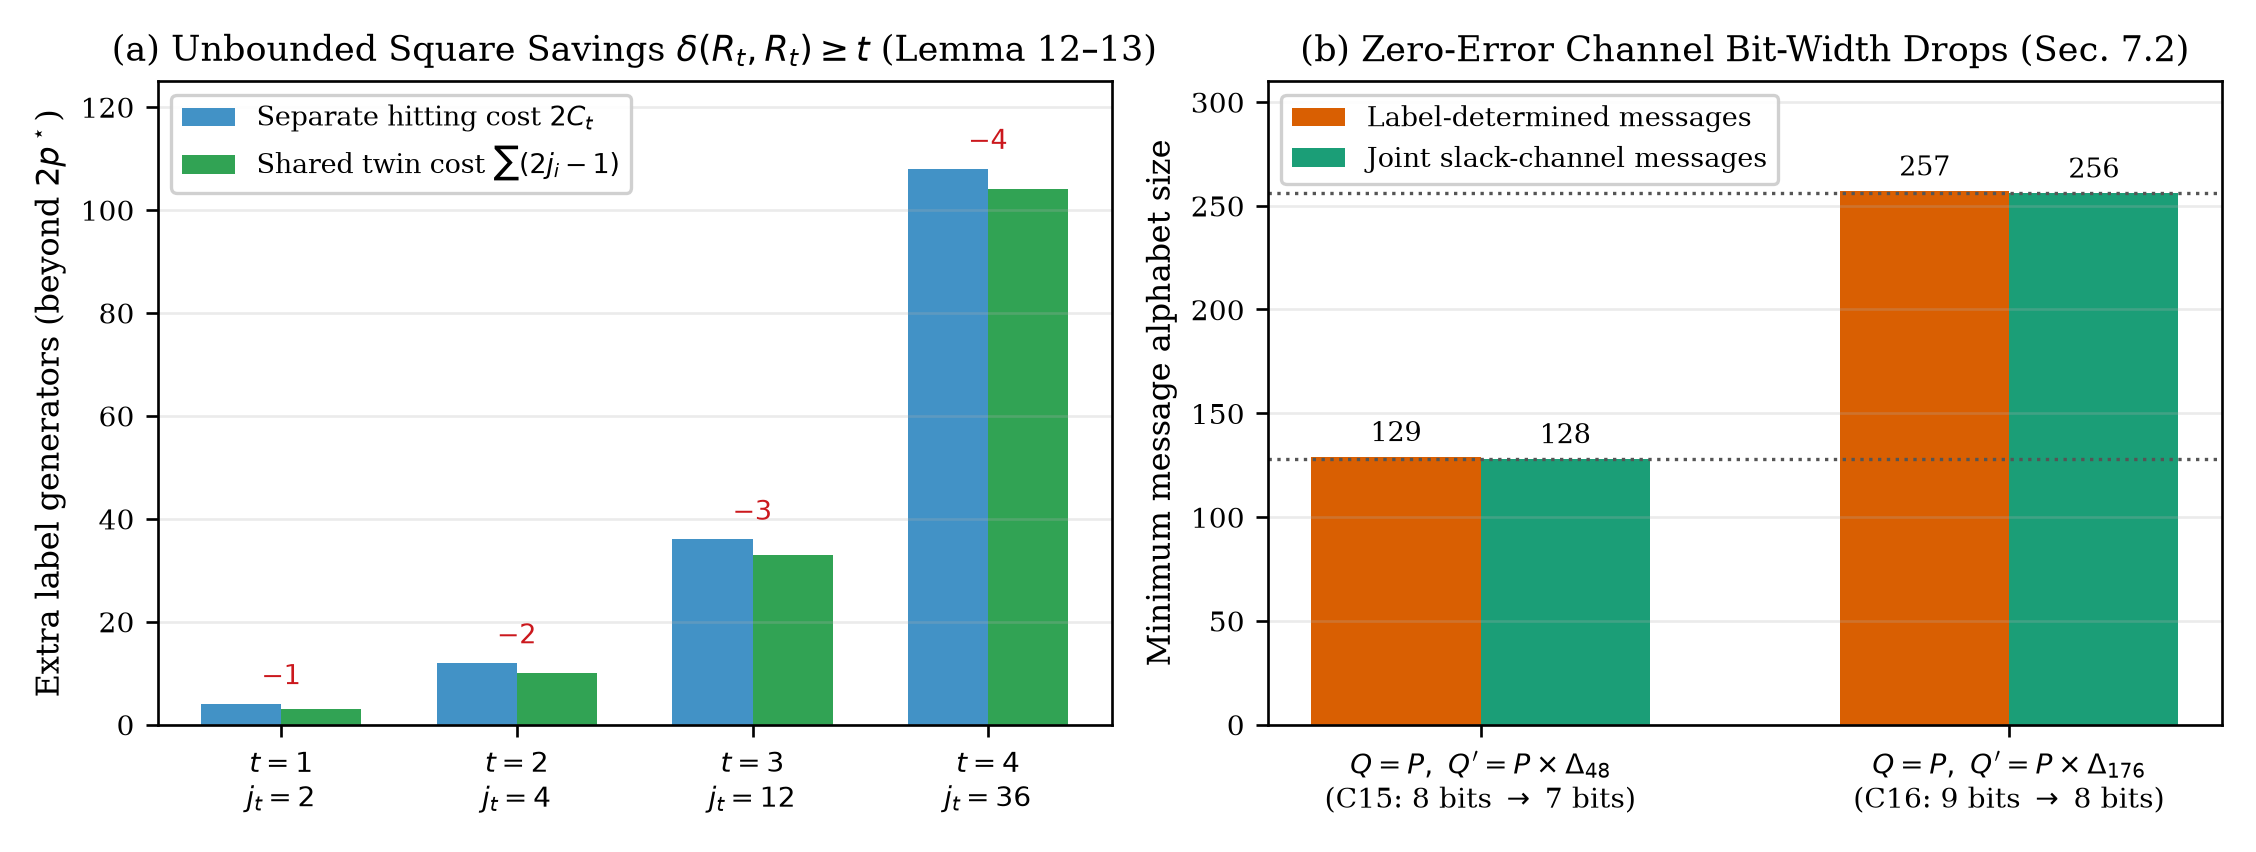
\includegraphics[width=0.90\textwidth]{figures/fig3_squares_and_channel_sim.png}
\caption{\textbf{Unbounded Cartesian Squares and Channel Simulation.} (a)~Canonical doubling sequence $j_1=2, j_i = 2\sum_{h<i}j_h$ yields exact saving $2C_t - \sum(2j_i-1) = t$ (Lemmas~12--13; live witnesses \texttt{C13}--\texttt{C14}). (b)~Zero-error slack-channel simulation achieves strict fixed-length bit-width drops in \texttt{C15} ($129\to 128$, $8\to 7$ bits) and \texttt{C16} ($257\to 256$, $9\to 8$ bits).}
\label{fig:fig3}
\end{figure*}

\paragraph{Worked Witness~1 (Polytope $P$ and Twin-Hexagon Matrix $S$, \texttt{C03}, \texttt{C05}, \texttt{C07}).}
At $L=10^6$, the 12-node twin-hexagon incidence matrix $R$ has exact $\mathbb{Q}$-rank $11$ and nullspace $\mathrm{span}(\kappa)$. Evaluating all 37 inequalities of Eq.~(5.2) of~\cite{Liu2026ExtensionComplexity} confirms 37 distinct facets and 39 vertices of $B\subset\mathbb{R}^{11}$: each of the 3 vertices $X_t$ has 1 positive omitted slack (the sum inequality, lifting to $2$ vertices) while each of the 36 vertices $X_t+LR_v$ has 2 positive opposite-pair slacks (lifting to $4$ vertices), yielding $3\cdot 2 + 36\cdot 4 = 150$ vertices and $24+26=50$ facets in dimension $11+13=24$ (\texttt{C03}). Meanwhile, \texttt{C05} certifies $\mathrm{rank}_{\mathbb{Q}}(S)=12$, verifies all $1{,}521$ columns of $S\otimes_1 S$ against the 27-generator dictionary $(R_v,0),(0,R_v),(A_s,A_s)$, and checks $D(R_v)=0, D(A_s)=D(X_t)=1$ on all 64 six-cycles, while \texttt{C07} certifies $\tau=1/5000 \implies \beta=1/200$, $\varepsilon=5201/10^6$, Claim~2 probe bound $663/2500$, and Claim~3 alternating bound $62412/76523$ (Fig.~\ref{fig:fig1}).

\paragraph{Worked Witness~2 (First Linear-Fraction Saving at $n=6$, \texttt{C09} \& \texttt{C11}).}
For $N=6$ ($p=72$ stars), Mode~3a (\texttt{C09}) confirms $1{,}080$ retained rows for $\Gamma_2$ ($\mathrm{rank}\,E_2=9$) and $1{,}728$ for $\Gamma_3$ ($\mathrm{rank}\,E_3=7$), with exact rank drop $1$ upon deleting every coarse node's incident edges. At $n=6$, Mode~3b (\texttt{C11}) verifies $\mathrm{rank}_+ M_{2,6} = 75\cdot 6 = 450$, $\mathrm{rank}_+ M_{3,6} \ge \lceil (72+\tfrac{32}{27})\cdot 6\rceil = 440$, and joint upper bound $(144+4)\cdot 6 = 888$, certifying $\delta(U_6, V_6) \ge 450+440-888 = 2 = \lceil 30/27\rceil$ (Fig.~\ref{fig:fig2}).

\paragraph{Worked Witness~3 (Unbounded Square $t=2$ and Zero-Error Channel Bit Saving, \texttt{C13} \& \texttt{C15}).}
For $j=[2,4]$ (\texttt{C13}), Mode~4a verifies $4\ge 2\cdot 2$, all $1{,}234$ pairwise intersections in $\mathcal{F}_2$ and $\mathcal{F}_4$, $C_2=6$, $N^\star = 20+4=24$, $p^\star = 24(6+140)=3{,}504$, and Lemma~13 scale $\sqrt{\Lambda}=10^{10}$, giving $\delta(R_2,R_2)\ge 2$. In \texttt{C15}, pairing $Q=P$ ($\mathrm{xc}=40$) with $Q'=P\times\Delta_{48}$ ($\mathrm{xc}=89$) reduces label-determined messages from $40+89=129$ ($8$ bits) to $\mathrm{xc}(P\times P\times\Delta_{48}) = 79+49=128 = 2^7$ ($7$ bits; Fig.~\ref{fig:fig3}b).

\section{Reproducibility and Availability}
All Lean~4 proofs, Python verifiers, certificates, figure scripts, and SHA-256 manifest (\texttt{MANIFEST.sha256}) are archived at \nolinkurl{https://github.com/lluiseriksson/extension-complexity-cartesian-certificates} under MIT (code/Lean/data) and CC-BY-4.0 (manuscript/figures) licenses. Reproduction requires three commands: \texttt{cd lean \&\& lake build}, \nolinkurl{python -m src.ext_complexity_verifier certificates}, and \texttt{pytest -q}.

\paragraph{AI Assistance Disclosure.}
Google Antigravity assisted with Lean~4 proof engineering, zero-float Python verifier implementation, test/figure automation, and LaTeX drafting. The author verified every mathematical derivation, Lean axiom audit, certificate check, and visual figure inspection, and takes full responsibility for all contents.

\bibliographystyle{plain}
\bibliography{references}
\end{document}
